\documentclass{standalone}
\usepackage{amsmath}
\usepackage{amssymb}
\usepackage{tikz}
\usepackage{mathrsfs}
\usepackage{ifthen}

\newcommand{\perpp}{\perp\!\!\!\perp}
\DeclareMathOperator{\so}{\mathfrak{s}}
\DeclareMathOperator{\ra}{\mathfrak{r}}
\DeclareMathOperator{\supp}{supp}
\DeclareMathOperator{\id}{id}
\DeclareMathOperator{\dom}{dom}
\DeclareMathOperator{\ran}{ran}
\DeclareMathOperator{\Min}{Min}
\DeclareMathOperator{\cod}{cod}
\newcommand{\smallerthan}{<}
\newcommand{\greaterthan}{>}
\newcommand{\defeq}{:=}
\newcommand{\eqdef}{=:}

\newcommand{\cat}[1]{\textbf{#1}}
\DeclareMathOperator{\IG}{\mathscr{IG}}


\begin{document}
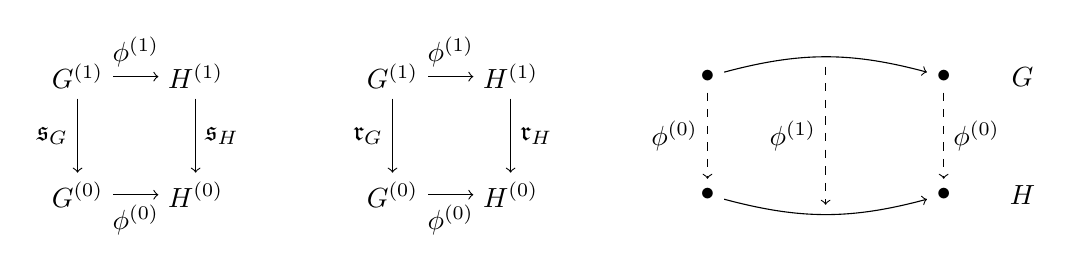
\begin{tikzpicture}
\node (G1) at (0,1) {$G^{(1)}$};
\node (G2) at ([shift={+(4,0)}]G1) {$G^{(1)}$};
\foreach \i in {1,2}
{\node (G\i2) at ([shift={+(1.5,0)}]G\i) {$H^{(1)}$};
\node (G\i3) at ([shift={+(0,-1.5)}]G\i) {$G^{(0)}$};
\node (G\i4) at ([shift={+(1.5,0)}]G\i3) {$H^{(0)}$};
\draw[->] (G\i)--(G\i2) node[above,midway] {$\phi^{(1)}$};
\draw[->] (G\i)--(G\i3) node[left,midway] {${\ifthenelse{\i=1}{\so}{\ra}}_G$};
\draw[->] (G\i3)--(G\i4) node[below,midway] {$\phi^{(0)}$};
\draw[->] (G\i2)--(G\i4) node[right,midway] {${\ifthenelse{\i=1}{\so}{\ra}}_H$};}
\node (G3) at ([shift={+(4,0)}]G2) {$\bullet$};
\node (G32) at ([shift={+(3,0)}]G3) {$\bullet$};
\node (G33) at ([shift={+(0,-1.5)}]G3) {$\bullet$};
\node (G34) at ([shift={+(0,-1.5)}]G32) {$\bullet$};
\draw[->] (G3) to[out=15,in=165] node[midway] (M1) {} (G32);
\draw[->] (G33) to[out=-15,in=195] node[midway] (M2) {} (G34);
\draw[->,dashed,thin] (M1)--(M2) node[midway,left] {$\phi^{(1)}$};
\draw[->,dashed,thin] (G3)--(G33) node[midway,left] {$\phi^{(0)}$};
\draw[->,dashed,thin] (G32)--(G34) node[midway,right] {$\phi^{(0)}$};
\node at ([shift={+(1,0)}]G32) {$G$};
\node at ([shift={+(1,0)}]G34) {$H$};


\end{tikzpicture}\end{document}